% !TEX program = XeLaTeX
% !TEX encoding = UTF-8
\documentclass{article}
 
\usepackage{xeCJK}
\setCJKmainfont{AozoraMinchoRegular.ttf}
\setCJKsansfont{KodomoRounded-Light.otf}
\setCJKmonofont{KodomoRounded-Light.otf}

\usepackage{url}
\usepackage{cancel}
\usepackage{xspace}
\usepackage{graphicx}
\usepackage{multicol}
\usepackage{multirow}
\usepackage{subfig}
\usepackage{amsmath}
\usepackage{amssymb}
\usepackage[a4paper, width=186mm, top=18mm, bottom=18mm, includeheadfoot]{geometry}
%\usepackage[a4paper, width=140mm, top=18mm, bottom=22mm, includeheadfoot]{geometry}
\usepackage{booktabs}
\usepackage{array}
\usepackage{verbatim}
\usepackage{caption}
\usepackage{natbib}
\usepackage{booktabs}
\usepackage{float}
\usepackage{pdflscape}
\usepackage{mathtools}
\usepackage[usenames, dvipsnames]{xcolor}
\usepackage{afterpage}
\usepackage{pgf}
\usepackage{tikz}
\usepackage{dirtree}
\usepackage[style=american]{csquotes}
\usepackage{amsfonts}
\usepackage{tikz}
\usepackage{tkz-graph}
\usetikzlibrary{arrows,decorations.pathmorphing,automata,positioning,backgrounds,fit,shapes.symbols,chains,intersections}

\newtheorem{definition}{Definition}[section]
\newtheorem{theorem}{Theorem}[section]
\newtheorem{lemma}{Lemma}
\newtheorem{proof}{Proof} [section]



\usepackage[toc, page, title, titletoc, header]{appendix}
\usepackage{marginnote}
\usepackage{tablefootnote}

%\renewcommand\appendixname{附\ 录}
%\renewcommand\appendixpagename{附\ 录}
%\renewcommand\appendixtocname{附\ 录}
\renewcommand\abstractname{Abstract}


\usepackage{perpage} %the perpage package
\MakePerPage{footnote} %the perpage package command

\usetikzlibrary{shapes.geometric}%
\usepackage{color}
%\usepackage[pages=some, placement=top]{background}
\usepackage{eso-pic}
\usepackage[final]{pdfpages}

%\includepdf[pages=1]{cover}
\hyphenpenalty=750

\title{\textbf{Loopring:}\\\textbf{分散型トークン取引所プロトコル}}
\author{
  Daniel Wang\\
  \texttt{daniel@loopring.org}\\
  \and
  	Jay Zhou\\
  	\texttt{jay@loopring.org}\\
  	\and
  	Alex Wang\\
  	\texttt{alex@loopring.org}\\
  	\and
  	Matthew Finestone\\
  	\texttt{matt.finestone@gmail.com}\\ 
  \\
  \texttt{https://loopring.org}
 }

\makeatletter
\def\CTEX@section@format{\Large\bfseries}
\makeatother

\makeatletter
\newenvironment{tablehere}
 {\def\@captype{table}}
 {}

\newenvironment{figurehere}
 {\def\@captype{figure}}
 {}
\makeatother
%
%\newcommand\BackgroundPic{%
%\put(0, 0){%
%\parbox[b][\paperheight]{\paperwidth}{%
%\vfill
%\centering
%\includegraphics[width=\paperwidth, height=\paperheight, %
%%keepaspectratio]{images/background.jpg}%
%]{images/background.jpg}%
%\vfill
%}}}


\begin{document}
%\AddToShipoutPicture{\BackgroundPic}
\maketitle


\begin{abstract}
Loopringは分散型取引所を構築するためのオープンプロトコルです。Loopringは、注文を集約し伝達するオフ・チェーンのアクターグループが集まり、注文の取引と決済の責任を負う一連のパブリックなスマートコントラクトとして機能します。プロトコルは自由で拡張性があり、交換機能を組み込んだ分散アプリケーション(dApp)用の標準化された構築用ブロックとして機能します。その相互運用可能な標準は、トラストレスな匿名取引を容易にします。現在の分散型取引所プロトコル上の重要な改善点は、2つのトークン取引ペアの制限を取り除き、異なるオーダー同士をミックスして一致させる能力であり、流動性を大幅に改善することです。Loopringではフロントランニング(オリジナルのソリューションプロバイダよりも早くブロックにトランザクションを登録する不公平な試行)を防止するための独自で頑強なソリューションを使っています。Loopringはブロックチェーンに依存せず、スマートコントラクト機能を備えたいかなるブロックチェーンにもデプロイすることができます。執筆時点では、イーサリアム\cite{buterin2017ethereum} \cite{wood2014ethereum}で動作可能であり、Qtum\cite{dai2017smart}、NEO\cite{atterlonn2018distributed}は準備中です。
\end{abstract}



\begin{multicols}{2}
\section{導入\label{sec:introduction}}

ブロックチェーンベースの資産が急増したため、取引相手との間でこれらの資産を交換する必要性が大幅に増加しました。従来の資産のトークン化を含む、何千もの新しいトークンが導入されているため、このニーズは拡大しています。投機的な取引を目的としたトークン交換、または、ネットワークへアクセスするためのネイティブなユーティリティトークンへの交換にかかわらず、1つの暗号資産を別の資産に交換する能力は、より大きなエコシステムの基礎になります。資産には潜在的なエネルギーが確かに存在\cite{desotocapital}しており、(資本を開放する)このエネルギーを実現するには、ブロックチェーンが永久に認めている所有権を主張するだけでなく、これらの資産を自由に移転し変換する能力が必要です。
 
そのため、トラストレスなトークン(価格)の交換は、ブロックチェーン技術の魅力的な使用例です。しかしながら、今では暗号通貨の熱心家は、伝統的な中央集権型取引所でのトークン取引で大部分を清算しています。Loopringが必要とされる理由として、Bitcoin\cite{nakamoto2008bitcoin}がピアツーピアの電子キャッシュに関して、「もし信頼できる第三者が以前として二重支払を防止する必要がある場合多くの利点が失われる」ことを忠実に強調したことと同様です。分散型資産もまた、信頼された、閉鎖的な中央集権型の取引所を通らなければならないのであれば、多くの利点が失われます。

中央集権型取引所上での分散型トークンの取引は、哲学的観点からは意味をなさない。なぜなら、これらの分散型プロジェクトが支持する長所を支えることができないからである。中央集権型取引所を使用する際には以下に説明されるように、多くの実用的なリスクと限界がある。分散型取引所(DEX)\cite{schuh2015bitshares} \cite{bancor} \cite{kyber}は、これらの問題に取り組むことを模索しており、多くの場合、直接取引のためにブロックチェーンを使用することによってセキュリティリスクを軽減することに成功している。”しかしながら、DEXの特性が新しい経済にとって重要なインフラストラクチャーになるにつれ、パフォーマンスの改善の余地はかなりあります。LoopringはdAppに依存しないオープンなプロトコルで、インフラストラクチャのための組み立て式ツールを提供することを目指しています。

\section{現在の取引所状況\label{sec:current_exchange_landscape}}

\subsection{中央集権型取引所の不十分さ}
中央集権型取引所の3つの主要なリスクは、1)安全性の欠如、2)透明性の欠如、3)流動性の欠如です。

\textbf{セキュリティの欠如}は、概して、ユーザーが自分の秘密鍵(資産)の制御をある中央集権型のエンティティに委譲することから発生します。これにより、ユーザーは中央集権型取引所が悪意のあるハッカーの餌食となる可能性にさらされます。すべての中央集権型取引所が直面するセキュリティとハッキングのリスクはよく知られていますが\cite{coincheckhack}  \cite{mcmillan2014inside}、未だにトークン取引において「当たり前のこと」としてよく受け入れられています。中央集権型取引所は、自身のサーバーに何百万ドルものユーザー資産を保有しているため、ハッカーにとって格好の的となり続けています。取引所の開発者は、ユーザーの資産で、過失的なエラーを引き起こすこともあります。簡単に言えば、ユーザーは中央集権型取引所に入金したときに自分のトークンの管理権限を失うことになります。  

\textbf{透明性の欠如}ユーザーを不正交換取引のリスクに不当にさらします。ここにおける特異性は取引所の悪意ある意図によるものであり、つまり中央集権型取引所においてユーザーは自身の資産を取引するというよりも、IOUを取引するということです。トークンが取引所のウォレットに送られると、その取引所に保管され、代わりにIOUとして提供します。そして、すべての取引は実質的にユーザーのIOUの間で行われます。出金するには、ユーザーは自身のIOUを償還し、トークンを外部ウォレットアドレスで受け取ります。これらの一連のプロセスは透明性が欠如しており、取引所が口座の停止、凍結、破産などを引き起こす可能性があります。また、ユーザーの資産が取引所の管理下にある間、それらの資産を第三者に貸し出すなど、他の目的で使用される可能性もあります。透明性の欠如は、取引手数料の増加、需要のピーク時の遅延、規制上のリスク、フロントランニング取引など、資産額の損失を生じさせることなく利用者を犠牲にする可能性があります。

\textbf{流動性の欠如。} 取引所の観点から、2つの勝者総取りのシナリオにより、断片化された流動性は新規取引所の参入を抑制します。一つ目のシナリオは、最も多くの取引ペアをもつ取引所が勝利するということです。なぜなら、ユーザーがすべての取引を一つの取引所で行うことが望ましいと感じるからです。二つ目のシナリオは、最も大きいオーダーブックを抱える取引所が勝利するということです。なぜなら、それぞれの取引ペアにおいて有利な売買スプレッドになるためです。これは新規参入者にとって初期の流動性を構築することが困難であるため、競争意欲を削いでしまいます。結果として、ユーザーからの苦情や大きなハッキング事件が起きてもなお、多くの取引所が高いマーケットシェアを持つこととなります。中央集権型の取引所は市場シェアを獲得するにつれて大きな価値を生むため、これまで以上に大きなハッキングの標的になります。

ユーザーの観点からは、断片化された流動性・換金能力はユーザー体験を大幅に低下させます。中央集権型の取引所では、ユーザーは取引所の流動性プールおよびオーダーブックの中でサポートされているトークンペア間でのみ取引することができます。トークン\verb|A|をトークン\verb|B|に交換するには、トークンを両方ともサポートする取引所に行くか、個人情報を開示して異なる取引所に登録する必要があります。ユーザは、通常、BTCまたはETHに対して予備的または中間的な取引をする必要があり、そのプロセスでは売買のスプレッドを支払う必要があります。最後に、オーダーブックは、注文した価格と実際に約定された価格差なしに取引を完了するのに十分な量がないかもしれません。たとえ取引所が大量処理を目的としていたとしても、この量と流動性が偽ではないという保証はありません\cite{fakevolume}。

その結果は古びた金融システムのように、流動性のないサイロと断片化されたエコシステムとなり、大きなボリュームが少数の取引所に集中します。ブロックチェーンのグローバルな流動性の保証は中央集権型取引所においてはメリットがありません。

\subsection{分散型取引所の不十分さ}
分散型取引所は中央集権型取引所とは異なり、ユーザーは基盤となるブロックチェーン上で直接的に取引を実行することによって自身の秘密鍵(資産)の管理を維持するからです。トラストレスな暗号化技術を活用することで、セキュリティを取り巻く上述のリスクの多くを首尾よく緩和します。しかしながら、性能及び構造上の限界に関して問題が依然として存在します。

流動性は、ユーザーが異なる流動性プールや標準を超えて取引相手を探す必要があるため、多くの場合問題となります。もし大規模なDEXやdAppsが相互運用するための一貫した標準を採用していない場合や、注文が幅広いネットワーク全体で共有/伝播されていない場合、断片的な流動性の影響は存在します。指値注文の流動性、具体的には、指値注文の再生成ーいかに早く指値注文を再注文できるかーは、最適なトレーディング戦略に大きな影響を及ぼしかねません\cite{limitorderliquidity}。そのような標準が存在しないことは、流動性の低下だけでなく、潜在的に安全性に欠ける独自のスマートコントラクトにさらされていることにもつながります。

さらに、オンチェーンで取引が行われるため、DEXはスケーラビリティ、実行の遅延(マイニング)、取引注文の変更に対するコストなど、基盤となるブロックチェーンの制限を継承します。したがって、ブロックチェーンのコードを実行するとコスト(ガス)が発生し、複数の注文取消は非常に高価になるため、ブロックチェーンのオーダーブックは特にうまく拡張できません。

最後に、ブロックチェーン上のオーダーブックは公開されているため、注文を行うトランザクションは、次のブロックで採掘されてオーダーブックに置かれるのを待っているので、マイナーから見えるようになります。この遅れは、ユーザーがフロントランニングの状態となるリスクと、思惑とは反する価格や取引執行が行われてしまうリスクにさらされます。

\subsection{ハイブリッドな解決策}
上記の理由から、純粋なブロックチェーンベースでの取引は制限を抱えており、中央集権型取引所と対抗させることはできません。オンチェーン固有のトラストレスであることと、中央集権型取引所の速さと注文の柔軟性との間にはトレードオフがあります。Loopringや0x\cite{warren20170x}のようなプロトコルは、オフチェーンでの注文管理とともにオンチェーンでの決済のソリューションを拡張しています。これらのソリューションは、オープンなスマートコントラクトを中心に展開されていますが、いくつかの機能をオフチェーンで実行し、ネットワークにとって非常に重要な役割を果たすノードに柔軟性を与えることによって、スケーラビリティの制限を回避します。しかし、ハイブリッドモデルにも欠点が残っています\cite{costofdecent}。Loopringプロトコルは、このホワイトペーパーを通じて我々のハイブリッドソリューションに対するアプローチにおける重要な違いを提案しています。

\section{Loopringプロトコル\label{sec:loopring_protocol}}
LoopringはDEXではなく、複数のブロックチェーンにDEXを構築するためのモジュラーなプロトコルです。我々は従来の取引所の構成部分を分解し、代わりにパブリックなスマートコントラクト群と分散したアクターを提供します。ネットワークの役割は、ウォレット、リレー、流動性共有コンソーシアムブロックチェーン、オーダーブックブラウザ、リングマイナー、アセットのトークン化サービスがあります。それぞれを定義する前に、我々は先ずLoopringにおける注文を理解する必要があります。

\subsection{オーダーリング\label{sec:order_ring}}
Loopringの注文は、一方向オーダーモデル(Unidirectional Order Model: UDOM)\cite{coinport2014udom}と呼ばれるもので説明されます。UDOMは、注文をトークンの交換リクエストとして、売り(Bid)と買い(Ask)ではなく、\verb|amountS|/\verb|amountB|(売る量/買う量)として表します。注文とはすべて、2つのトークン間の交換レートにすぎないため、サーキュラートレードでの複数の注文を混ぜ合わせマッチングさせることが、プロトコルの強力な特徴となります。一組の取引ペアの代わりに、最大16の注文を使うことで、流動性と価格上昇の可能性が劇的に増大します。

\begin{center}
\begin{figurehere}
\centering
\tikzstyle{block} = [draw, fill=blue!20, rectangle, 
    minimum height=3em, minimum width=6em]
\tikzstyle{sum} = [draw, fill=blue!20, circle, node distance=1cm]
\tikzstyle{input} = [coordinate]
\tikzstyle{output} = [coordinate]
\tikzstyle{pinstyle} = [pin edge={to-,thin,black}]

\begin{tikzpicture}[
    auto, 
    node distance=2cm,
    >=latex',
    font=\bfseries\footnotesize\sffamily,
    order/.style={
		scale=0.7,
		rectangle,
		rounded corners,
		draw=black, 
		text centered,
%		text width=5cm,
		minimum height=12mm,
		fill=white
	},
	label/.style={
		scale=0.7
	}
  ]
    % We start by placing the blocks

  \node [order] (order2) 
 {%
 \begin{tabular}{l}
  \textbf{注文\#2}\\
  \textbf{所有者: Y}\\
  \textbf{amountS: 9B}\\
  \textbf{amountB: 12C}
 \end{tabular}
 };
 
  \node [order, below of=order2, xshift=-3.5cm] (order1) 
 {%
 \begin{tabular}{l}
  \textbf{注文\#1}\\
  \textbf{所有者: X}\\
  \textbf{amountS: 10000A}\\
  \textbf{amountB: 2B}
 \end{tabular}
 };
 
 
  \node [order, below of=order2, xshift=3.5cm] (order3) 
 {%
 \begin{tabular}{l}
  \textbf{注文\#3}\\
  \textbf{所有者: Z}\\
  \textbf{amountS: 100C}\\
  \textbf{amountB: 160A}
 \end{tabular}
 };
 
 \draw [draw,->] (order1) -- node [label] {\textbf{7898A}} (order3);
 \draw [draw,->] (order2) -| node [label, xshift=-1.8cm] {\textbf{8B}} (order1);
 \draw [draw,->] (order3) |- node [label, xshift=1cm, yshift=0.24cm] {\textbf{98C}} (order2);

\end{tikzpicture}

\caption{3つの注文のオーダーリング}
\label{fig:ring}
\end{figurehere}
\end{center}


上の図は3つの注文のオーダーリングです。各注文の売却するトークン(\verb|tokenS|)は、別の注文の購入するトークン(\verb|tokenB|)です。これは、各注文が、対となるトークンのペアを必要とせずとも、欲しいトークンと交換することを可能にするループを作成します。本質的にはオーダーリングの特別なケースとなるが、従来のペアトレードの注文も、もちろん実行可能です。

\begin{definition}[オーダーリング] $C_{0}$, $C_{1}$, $\cdots$, $C_{n-1}$が、$n$種類のトークンとし、$O_{0\rightarrow 1}$, $\cdots$, $O_{i\rightarrow i\oplus 1}$, $\cdots$, $O_{n-1 \rightarrow 0}$が$n$種類の注文とします。このとき、注文はオーダーリングを作り、取引可能になります。
$$O_{0\rightarrow 1} \rightarrow \cdots \rightarrow O_{i\rightarrow i\oplus 1} \rightarrow \cdots \rightarrow O_{n-1\rightarrow 0} \text{, }$$
$n$がオーダーリングの長さだとすると、$i\oplus 1 \equiv i+1$を$n$で割った余りは等しくなります。
\end{definition}

オーダーリングが成立するのは、すべての構成トランゼクションが、ユーザーが明示的に指定した元々のレートと同等、もしくはより良いレートで取引されるときです。オーダーリングの成立を確認するためには、Loopringスマートコントラクトは、すべての注文の元々の交換レートが、1に等しいか1より大きいオーダーリングを、リングマイナーから受け取らなければなりません。

アリスとボブがトークン\verb|A|とトークン\verb|B|を交換したがっているとしましょう。アリスは15トークン\verb|A|をもっていて、その対価に4トークン\verb|B|が欲しく、ボブは10トークン\verb|B|もっていて、その対価に30トークン\verb|A|が欲しいとします。

誰が買い、誰が売るのでしょうか?これは価格相場によってのみ決定されます。トークン\verb|A|を固定して考えるのであれば、アリスはトークン\verb|B|を、${15 \over 4} = 3.75$\verb|A|の価格で買い、ボブは10トークン\verb|B|を、${30 \over 10} = 3.00$\verb|A|で売ります。トークン\verb|B|を固定して考えるのであれば、アリスは15トークン\verb|A|を、${4\over 15}=0.26666667$\verb|B|の価格で売り、ボブはトークン\verb|A|を${10 \over 30}=0.33333334$\verb|B|の価格で買います。つまり、誰が買って誰が売るかは恣意的なものなのです。

最初のシチュエーションでは、アリスは、ボブが売る価格($3.00$\verb|A|)よりも高い価格($3.75$\verb|A|)で買おうとしています。次のシチュエーションでは、ボブは、アリスが売る価格($0.26666667$\verb|B|)よりも高い価格($0.33333334$\verb|B|)で買おうとしています。買う側が、売値と同じか高い価格で買おうとするとき、取引は常に成立するのです。

\begin{equation}
{{15\over 4} \over {30\over 10}} = {{10\over 30} \over {4\over 15}}={15 \over 4} \cdot {10 \over 30} = 1.25 > 1
\end{equation}

したがって、$n$個の注文が処理されるには、完全であれ、部分的であれ、買い注文の各交換レートの結果が1と同じ、或いはそれを上回っているかを知る必要があります。もしそうであれば、$n$個の注文は完全に、もしくは部分的に処理がなされます。\cite{supersymmetry}

仮に第三の人物であるチャーリーを持ち出してみると、アリスは$x_1$トークン\verb|A|を手放し$y_1$トークン\verb|B|を受け取り、ボブは$x_2$トークン\verb|B|を手放し$y_2$トークン\verb|C|を受け取り、チャーリーは$x_3$トークン\verb|C|を手放し$y_3$トークン\verb|A|を受け取ることになります。必要なトークンが存在するとした場合、取引は次のとき成立します。

\begin{equation}
{{x1 \cdot x_2 \cdot x_3 \over y_1 \cdot y_2 \cdot y_3} \geq 1}
\end{equation}


Loopringの注文の詳細についてはセクション\ref{anatomy}を参照してください。



\section{エコシステム参加者\label{sec:ecosystem}}
以下のエコシステム参加者は、協同することで、中央集権の取引所が備える全ての機能を提供します。

\begin{itemize}

\item \textbf{ウォレット}: トークンへのアクセスや、Loopringネットワークへの注文の送信を、ユーザーが行えるようにする一般のウォレットサービスおよびインターフェースです。ウォレットには、リングマイナーと手数料を分け合うことで、注文を生成するインセンティブが生まれます。(セクション\ref{sec:token}を参照。)取引の将来は、個々のユーザーのウォレットの安全性が確保された中で行われるという考えに立つと、これらの流動性プールを我々のプロトコルで繋げることが最良となるのです。

\item \textbf{コンソーシアム型流動性共有ブロックチェーン/リレーメッシュ}: 注文と流動性共有のためのリレーメッシュネットワークです。ノードがLoopringのリレーソフトウェアを実行すると、既存のネットワークに接続し、コンソーシアム型のブロックチェーンを介して他のリレーと流動性を共有することができます。最初の実装として我々が構築しているコンソーシアム型ブロックチェーンは、ほぼリアルタイムのオーダー共有機能(1-2秒のブロック)を持ち、古い記録を削除することで新たなノードの高速なダウンロードを可能にします。ノードはこのコンソーシアムに接続しないこともできます。流動性を共有せず独立を保ったり、あるいは独自の流動性共有ネットワークを立ち上げることもできます。

\item \textbf{リレー/リングマイナー}: リレーはウォレットやリレーメッシュから注文を受け取るノードで、公のオーダーブックと取引履歴を維持し、任意に他のリレー(オフチェーン媒体を介して)および/またはリレーメッシュノードに注文をブロードキャストします。リングマイニングはリレーの特徴であり、必要条件ではありません。リングマイニングは計算負担が高く、完全にオフチェーンで行われます。私達はリングマイニングの特徴を有するリレーを「リングマイナー」と呼び、リングマイナーは全く異なる注文をつなぎ合わせてオーダーリングを作ります。リレーは、(1)それらが相互に通信する方法、(2)オーダーブックを作成する方法、(3)オーダーリングをマイニング(マイニングアルゴリズム)する方法は自由です。

\item \textbf{Loopringプロトコルスマートコントラクト (LPSC)}: リングマイナーから受信したオーダーリングをチェックし、ユーザーに代わりトークンをトラストレスに決済および交換し、リングマイナーとウォレットへ報酬を与え、イベントを発生させる、公開された自由なスマートコントラクトのセットです。 リレー/オーダーブラウザは、これらのイベントを監視し、オーダーブックと取引履歴を最新の状態に保ちます。詳細については、付録\ref{app:protocol_ethereum}を参照してください。

\item \textbf{資産トークン化サービス (ATS)}: Loopring上で直接取引することが出来ない資産の橋渡し。これらは信頼のできる会社もしくは組織によって中央集権化されたサービスです。ユーザーは資産(現物、通貨あるいは他のチェーンからのトークン)を預金し、トークンを発行します。これは将来、預けた資産と引き換えられます。Loopringは(適切な解決策が存在するまで)クロスチェーン取引プロトコルではありませんが、ATSはERC20トークン\cite{ERC20}の取引を、他のブロックチェーン上の資産だけでなく物理資産でも可能にします。

\end{itemize}


\section{取引プロセス\label{sec:process}}



\begin{enumerate} 


\item \textbf{プロトコル権限}: 図\ref{fig:process}において、トークンを交換したいユーザー\verb|Y|は自身が売却したいトークン\verb|B|の\verb|amountS|を処理するようLPSCに許可します。これにより、ユーザーのトークンはロックされず、注文が処理されるまでトークンを自由に動かすことができます。

\item \textbf{注文作成}: トークン\verb|B|とトークン\verb|C|の現在のレートとオーダーブックは、リレーもしくはオーダーブックブラウザのようなネットワークに繋がっている他のエージェントによって提供されます。ユーザー\verb|Y|は、任意の統合されたウォレットのインターフェースを介して特定の\verb|amountS|、\verb|amountB|、または他のパラメーターの注文(指値)を置きます。LRxはリングマイナーへの手数料として注文に加えることができます。より高いLRx手数料はリングマイナーによって早く処理されるより良い機会を与えます。注文のハッシュはユーザー\verb|Y|の秘密鍵で署名されます。

\item \textbf{注文のブロードキャスト}: ウォレットは一つあるいは複数のリレーに注文と署名を送信します。リレーは公開されているオーダーブックを更新します。プロトコルは、先入れ先出しのように、ある一定の方法でオーダーブックを作成することを要求しません。代わりに、リレーはオーダーブックを作成する際に、独自の設計上の決定を下す権限を持っています。

\item \textbf{流動性の共有}: リレーは任意の通信媒体を介して他のリレーにオーダーをブロードキャストします。また、ノードがどのように相互作用するかについては柔軟性があります。一定レベルのネットワーク接続を容易にするために、コンソーシアムブロックチェーンを使用した組み込みの流動性共有のためのリレーメッシュが存在します。前のセクションで述べたように、このリレーメッシュは速度と包括性のために最適化されています。

\begin{center}
\begin{figurehere}
\centering
\tikzstyle{block} = [draw, fill=blue!20, rectangle, 
    minimum height=3em, minimum width=6em]
\tikzstyle{sum} = [draw, fill=blue!20, circle, node distance=1cm]
\tikzstyle{input} = [coordinate]
\tikzstyle{output} = [coordinate]
\tikzstyle{pinstyle} = [pin edge={to-,thin,black}]

\begin{tikzpicture}[
    auto, 
    scale=0.7,
    node distance=2cm,
    >=latex',
    font=\bfseries\footnotesize\sffamily,
    order/.style={
		rectangle,
		scale=0.7,
		rounded corners,
		draw=black, 
		text centered,
%		text width=5cm,
		minimum height=12mm,
		minimum width=30mm,
		fill=white
	},
	role/.style={
		circle,
		scale=0.7,
		draw=black, 
		text centered,
%		text width=5cm,
		minimum height=12mm,
		minimum width=12mm,
		fill=white
	},
	steps/.style={
		circle,
		scale=0.7,
		draw=black, 
		text centered,
%		text width=5cm,
%		minimum height=12mm,
%		minimum width=12mm,
		fill=black,
		text=white
	},
	account/.style={
		circle,
		scale=0.7,
		draw=black, 
		text centered,
%		text width=5cm,
		minimum height=16mm,
		minimum width=16mm,
		fill=white
	},
	label/.style={
	  scale=0.7
    }
  ]

 
 \node [role] (user1)  {ユーザー X};
 \node [role, below of=user1] (user2)  {ユーザー Y};
 \node [role, below of=user2] (user3)  {ユーザー Z};
 \node [role, below of=user3, fill=gray!20] (relay1)  {リレー M};
 \node [role, below of=relay1, fill=gray!20] (relay2)  {リレー N};

 
 \node [order, left of=user1, xshift=-1cm] (order1) 
 {%
 \begin{tabular}{l}
  \textbf{注文\#1}\\
  \textbf{所有者: X}\\
  \textbf{amountS: 10000 A}\\
  \textbf{amountB: 2 B}
 \end{tabular}
 };
 
 \draw [draw, ->]  (user1) -- (order1) [label]{};
 \draw [bend right,->] (order1) to node [auto, scale=0.7] {} (relay1);
 \draw [bend right,->] (order1) to node [auto, scale=0.7] {} (relay2);
% \draw [draw, ->]  (order1) |- (relay1) [label]{};
% \draw [draw, ->]  (order1) |- (relay2) [label]{};
 
 \node [order,left of=user2, xshift=-1.5cm] (order2) 
 {%
 \begin{tabular}{l}
  \textbf{注文\#2}\\
  \textbf{所有者: Y}\\
  \textbf{amountS: 9  B}\\
  \textbf{amountB: 12 C}
 \end{tabular}
 };
 \draw [draw, ->]  (user2) -- (order2) [label]{};
 \draw [bend right,->] (order2) to node [auto, scale=0.7] {} (relay1);
 \draw [bend right,->] (order2) to node [auto, scale=0.7] {} (relay2);
% \draw [draw, ->]  (order2) |- (relay1) [label]{};
% \draw [draw, ->]  (order2) |- (relay2) [label]{};
% 
\node [order, left of=user3, xshift=-2cm] (order3) 
 {%
 \begin{tabular}{l}
  \textbf{注文\#3}\\
  \textbf{所有者: Z}\\
  \textbf{amountS: 100 C}\\
  \textbf{amountB: 160 A}
 \end{tabular}
 };
 \draw [draw, ->]  (user3) -- (order3) [label]{};
 \draw [bend right,->] (order3) to node [auto, scale=0.7] {} (relay1);
 \draw [bend right,->] (order3) to node [auto, scale=0.7] {} (relay2);
% \draw [draw, ->]  (order3) |- (relay1) [label]{};
% \draw [draw, ->]  (order3) |- (relay2) [label]{};
 
% // The Ring
\node [order, 
yshift=-1.5cm,
xshift=-2.75cm,
below of=relay2,
fill=gray!10,
minimum width=4.2cm,
minimum height=5cm] (ring) {};


\node [order, dashed, below of=relay2,yshift=-0.2cm,xshift=-2.5cm] (order11) 
 {%
 \begin{tabular}{l}
  \textbf{注文\#1}\\
  \textbf{所有者: X}\\
  \textbf{amountS: 10000 A}\\
  \textbf{amountB: 2 B}
 \end{tabular}
 };
 \node [order, dashed,below of=order11,xshift=-0.25cm,yshift=0.7cm] (order21) 
 {%
 \begin{tabular}{l}
  \textbf{注文\#2}\\
  \textbf{所有者: Y}\\
  \textbf{amountS: 9  B}\\
  \textbf{amountB: 12 C}
 \end{tabular}
 };
\node [order, dashed,below of=order21,xshift=-0.25cm,yshift=0.7cm] (order31) 
 {%
 \begin{tabular}{l}
  \textbf{注文\#3}\\
  \textbf{所有者: Z}\\
  \textbf{amountS: 100 C}\\
  \textbf{amountB: 160 A}
 \end{tabular}
 };
 
 % // The blockchain
\node [
rectangle,
fill=gray!20, 
right of=user1,
yshift=-4.5cm,
xshift=0.1cm,
scale=0.7,
minimum width=3.2cm,
minimum height=15.6cm] (blockchain) {\parbox[b][15cm]{1.3cm}{ブロックチェーン}};
% blockchain accounts
  \node [account, right of=user1, xshift=1cm] (account1)  {accountX};
  \node [account, right of=user2, xshift=1cm] (account2)  {accountY};
  \node [account, right of=user3, xshift=1cm] (account3)  {accountZ};
  \node [account, right of=relay1, xshift=1cm] (account4)  {accountM};
  \node [account, right of=relay2, xshift=1cm] (account5)  {accountN};
  \node [account, double, below of=account5, yshift=-1.5cm] (psc)  {LPSC};
  
 \draw [draw, ->]  (user1) -- (account1) [label]{};
 \draw [draw, ->]  (user2) -- (account2) [label]{};
 \draw [draw, ->]  (user3) -- (account3) [label]{};
% \draw [draw, ->]  (relay1) -- (account4) [label]{};
% \draw [draw, ->]  (relay2) -- (account5) [label]{};
 \draw [draw, double, thick]  (relay1) to node [auto, scale=0.7] {流動性を共有する}  (relay2) [label]{};
% \draw [draw, ->]  (relay1) -- (ring) [label]{};
 \draw [draw, ->]  (relay2) to node [auto, scale=0.7, xshift=-1.8cm, yshift=0.3cm] {リングマイニング}  (ring) [label]{};
 \draw [draw, ->]  (ring) to node [auto, scale=0.7] {submitRing} (psc) [label]{};
 
 \draw [bend left,->] (account1) to node [auto, scale=0.7] {\textbf{7898 A}} (account3);
 \draw [bend left,->] (account2) to node [auto, scale=0.7] {\textbf{8 B}} (account1);
 \draw [bend left,->] (account3) to node [auto, scale=0.7] {\textbf{98 C}} (account2);
 
 \draw [bend left,->, dashed] (account1) to node [auto, scale=0.7] {} (account5);
 \draw [bend left,->, dashed] (account2) to node [auto, scale=0.7] {} (account5);
 \draw [bend left,->, dashed] (account3) to node [auto, scale=0.7, xshift=.5cm] {\textbf{手数料}} (account5);
  
  
% \draw [draw,->] (order1) -- node [label] {\textbf{7898 A}} (order3);
% \draw [draw,->] (order2) -| node [label, xshift=-1.8cm] {\textbf{8 B}} (order1);
% \draw [draw,->] (order3) |- node [label, xshift=1cm, yshift=0.24cm] {\textbf{98 C}} (order2);

\node [steps, right of=user2, xshift=-0.6cm] () {1};
\node [steps, left of=user2, xshift=0.8cm] () {2};
\node [steps, left of=relay2, xshift=0.3cm, yshift=1cm] () {3};
\node [steps, left of=relay1, xshift=3.3cm, yshift=-1.6cm] () {4};
\node [steps, below of=relay2, xshift=-0.2cm, yshift=0.4cm] () {5};
\node [steps, right of=account3, xshift=-0.6cm] (step5) {6};

 \draw [bend right, ->]  (psc) to node [auto, scale=0.7, xshift=0.5cm] {決済処理} (step5) [label]{};
 
\end{tikzpicture}

\caption{Loopring取引プロセス}
\label{fig:process}
\end{figurehere}
\end{center}



\item \textbf{リングマイニング(注文マッチング)}: リングマイナーは、注文を複数の他の注文と照合することで、指定された為替レートまたは、より良いレートで完全または部分的に記入しようとします。プロトコルがどんなペアよりも高い流動性を提供することができる主な理由はリングマイニングです。もし実行されたレートがユーザ Y が指定したレートよりも良い場合は、オーダーリング内のすべての注文間でマージンが共有されます。報酬としてリングマイナーは、マージンの部分(マージンスプリット、そしてLRxトークンをユーザーに返す)を請求するか、単にLRx料金を維持するかを選択します。

\item \textbf{検証\&決済}: オーダーリングはLPSCによって受け取られます。リングマイナーが提供するデータを検証するための複数のチェックを行い、オーダーリングが完全にまたは部分的に決済することができるかどうかを決定します(ユーザーウォレット内のトークンおよびリング内の注文の記入割合によって決定します)。もしすべてのチェックが成功している場合、コントラクトはユーザーにアトミック(完全に行なわれるか全く行なわれないかのいずれか)にトークンを転送し、リングマイナーとウォレットに手数料を同時に支払います。LPSCによって決定されたユーザ\verb|Y|の残高が不十分な場合、注文自体がスケールダウンされたものとみなされます:キャンセルはされず、アドレスに十分な資金が入金された場合、スケールダウンした注文は自動的に元のサイズに拡大されます。これは一方通行の手動操作であり、元に戻すことはできません。


\end{enumerate}





%
%\end{multicols}
%
%\begin{center}
%\begin{figurehere}
%\includegraphics[height=8cm]{images/en_protocol.png}
%\caption{Loopring Trading Process}
%\label{fig: Loopringrotocol}
%\end{figurehere}
%\end{center}
%
%\begin{multicols}{2}

\section{オペレーションの柔軟性\label{sec:business_model}}
Loopringのオープンスタンダードにより、参加者のオペレーションには大きな柔軟性が提供されることに注意することが重要です。参加者は新しいビジネスモデルを自由に構築してユーザーに価値を提供し、取引量やその他の基準でLRx手数料を得ることも、(もしそう選べば)可能なのです。エコシステムはモジュール式になっており、多様なアプリケーションからの参加者をサポートするようにできています。


\subsection{オーダーブック\label{sec:order_book}}
リレーは、ユーザーの注文を表示して一致させるために、多数の方法でオーダーブックを設計することができます。我々自身の最初のオーダーブックはOTCモデルを採用しており、価格のみに基づいて指値のポジションがとられます。言い換えれば、注文のタイムスタンプは、オーダーブックとは関係がありません。しかしながらリレーは、自由にオーダーブックを設計することができるため、典型的な中央集権型の取引所のマッチングエンジンをまねて注文を価格順に並べる一方、同時にタイムスタンプも考慮する、といったことも可能です。リレーがこのようなオーダーブックを提供する場合、内部にウォレットを保持あるいは組み込み、ウォレットの注文を単独のリレーに送り、タイムスタンプに基づいて注文をマッチさせます。このような構成も可能となっています。


他のDEXプロトコルの中には、リレーにリソース(テイカーが注文を出すための初期トークン残高)が必要なものがあるのに対し、Loopringリレーは、マッチして取引を成立させる注文を見つけるのみでよいため、初期トークンなしで行うことができます。

\subsection{流動性の共有\label{sec:liquidity_sharing}}
リレー同士は、いかに流動性(注文)を互いに共有するかの設計も自在にできます。我々のコンソーシアム型ブロックチェーンは、これを成し遂げるソリューションであり、エコシステムは望むままにネットワークに接続し交流することが可能です。コンソーシアム型ブロックチェーンに接続する以外にも、独自のものを構築・管理することができ、各々に合うルール/インセンティブを加えることができます。リレーは独立して稼働することもできます。時間が重要な要素となるウォレットの実装などがその例です。もちろん、ネットワーク効果を追求する上では、他のリレーと交流することに明確な優位性がありますが、異なるビジネスモデル間では、特定の共有設計において手数料を共有するほうがメリットが大きいこともありえます。


\section{プロトコルの特徴\label{sec:protocol}}

\subsection{注文の詳細\label{anatomy}}
注文とは、ユーザーの取引の意図を示すデータの集まりです。Loopringでの注文は、一方向オーダーモデル、すなわちUDOMを使うことで、以下のように定義されます。

\begin{verbatim}
  message Order {
    address protocol;
    address owner;
    address tokenS;
    address tokenB;
    uint256 amountS;
    uint256 amountB;
    unit256 lrcFee
    unit256 validSince; // 基準時点からの通算秒
    unit256 validUntil; // 基準時点からの通算秒
    uint8   marginSplitPercentage;  // [1-100]
    bool    buyNoMoreThanAmountB;
    uint256 walletId;
    // 二重認証アドレス
    address authAddr;
   	// v, r, sは署名のパーツ
    uint8   v;       
    bytes32 r;
    bytes32 s;
    // 二重認証するプライベートキー。
    // オーダーのハッシュ計算には使用されないため、
    // 署名されない。
    string  authKey;          
  }
\end{verbatim}


注文の発信元を保証するため、\verb|authAddr|を除くパラメーターのハッシュに対してユーザーの秘密鍵で署名します。 \verb|authAddr|パラメーターは、この注文の一部であるオーダーリングに署名するために使用され、フロントランニングを防止します。詳細はセクション9.1を参照してください。署名は、\verb|v|、\verb|r|、および\verb|s|フィールドで表され、ネットワークを介して注文パラメータとともに送信されます。 これにより、注文は完了するまで不変であることが保証されます。注文が不変であっても、プロトコルは他の変数と一緒にアドレスの残高に基づいて現在の状態を計算することが可能です。


UDOMは(性質的に浮動小数点数でなければならない)価格を含んでいませんが、代わりに、\verb|amountS|/\verb|amountB|で表される\verb|rate|または$r$という用語が使用されます。レートは浮動小数点数ではなく、要求により他の符号なし整数で評価されるものですが、これにより、中間結果が符号なし整数のままとなり、計算の正確性が増します。


\subsubsection{購入量}

リングマイナーが注文をリングマッチさせるとき、より良いレートで取引が行われ、ユーザーが指定した\verb|amountB|よりも多くの\verb|tokenB|を手にすることは起こりえます。しかしながら、もしも「\verb|amountB|以上は買わない」が真と設定されれば、ユーザーが\verb|amountB|以上の\verb|tokenB|を手にしないよう、プロトコルは保証します。このように、UDOMの\verb|buyNoMoreThantokenB|パラメータにより、注文が完全に処理されたと考えられる時期が決まるのです。\verb|buyNoMoreThantokenB|は\verb|amountS|にも\verb|amountB|の上限にもあてはまり、伝統的な買い/売りの注文よりもきめ細かいユーザーの取引の意図を反映可能になります。

例えば、\verb|amountS|が10で\verb|amountB|が2の場合、レート$r$ = 10/2 = 5となります。ユーザーは各\verb|tokenB|に対し5つの\verb|tokenS|を売るつもりということになります。リングマイナーがレート4のユーザーを見つけてマッチすれば、そのユーザーは2ではなく2.5の\verb|tokenB|を得ることができます。しかしながら、そのユーザーが2つの\verb|tokenB|しか欲しくなく、\verb|buyNoMoreThanAmountB|フラグを\verb|True|と設定していた場合、LPSCはレート4にて作用し、ユーザーは各\verb|tokenB|に対し4つの\verb|tokenS|を売り、2つの\verb|tokenS|を節約します。これは、マイニング手数料を考慮していないことに留意してください。(セクション\ref{sec:fee_model}を参照してください。)

実際に、


\begin{verbatim}
	      Order(amountS,tokenS,
	            amountB,tokenB,
	            buyNoMoreThantokenB)
\end{verbatim}

を使用して注文を簡素化した形式で表すと、従来の取引所でのETH/USDマーケットにおいて、従来の購入-売却モデルでは下の1番目と3番目の注文は表現できますが、他の2つは表現することができません。

\begin{enumerate}
	\item 10 ETHを 300 USD/ETH の価格で売る。この注文は次のように表されます:\verb|Order(10, ETH, 3000, USD, False)|。
	\item 1 ETHを 300 USD/ETH の価格で売り 3000 USD を得る。この注文は次のように表されます:\verb|Order(10, ETH, 3000, USD, True)|。
	\item 10 ETHを 300 USD/ETH の価格で買う。この注文は次のように表されます:\verb|Order(3000, USD, 10, ETH, True)|。
	\item 3000 USD で買える限りの ETH を 300 USD/ETH の価格で買う。この注文は次のように表されます:\verb|Order(3000, USD, 10, ETH, False)|。
\end{enumerate}



\subsection{リング検証\label{sec:ring_verification}}

Loopringのスマートコントラクトは、交換レートや取引量の計算は行いませんが、リングマイナーが取引で提示するこれらの情報を受け取り、検証しなければなりません。これらの計算は、以下の2つの理由により、リングマイナーの手でなされます。(1)イーサリアムでのsolidity\cite{dannen2017introducing}のような、スマートコントラクト用のプログラミング言語は、浮動小数点数、$pow(x, 1/n)$(浮動小数点数のn乗根の計算)をサポートしておらず、(2)ブロックチェーンの処理量とコストを削減するには、処理がオフチェーンで行われたほうが望ましいためです。


\subsubsection{サブリングチェック\label{sec:sub_ring_check}}
このステップにより、アービトラージをする取引者が、新規の注文を実行してオーダーリング内のマージンを不当に得ることを防止します。リングマイナーが、オーダーリングが有効となったのを確認すると、他の注文をオーダーリングに加えてユーザーのマージン(レートディスカウント)を全て得ようという誘因が本質的に生まれます。下の図\ref{fig:subring}で表されるように、注意深く計算された場合には、$x1$, $y1$, $x2$, $y2$は注文のレート結果はちょうど1となり、レートディスカウントは発生しません。

\begin{center}
\begin{figurehere}
\centering
\tikzstyle{block} = [draw, fill=blue!20, rectangle, 
    minimum height=3em, minimum width=6em]
\tikzstyle{sum} = [draw, fill=blue!20, circle, node distance=1cm]
\tikzstyle{input} = [coordinate]
\tikzstyle{output} = [coordinate]
\tikzstyle{pinstyle} = [pin edge={to-,thin,black}]

\begin{tikzpicture}[
    auto, 
    node distance=2cm,
    >=latex',
    font=\bfseries\footnotesize\sffamily,
    order/.style={
		scale=0.7,
		rectangle,
		rounded corners,
		draw=black, 
		text centered,
%		text width=5cm,
		minimum height=12mm,
		fill=white
	},
	label/.style={
		scale=0.7
	}
  ]
    % We start by placing the blocks

  \node [order] (order2) 
 {%
 \begin{tabular}{l}
  \textbf{注文\#2}\\
  \textbf{所有者: Y}\\
  \textbf{amountS: 9B}\\
  \textbf{amountB: 12C}
 \end{tabular}
 };
 
  \node [order, below of=order2, xshift=-3.5cm] (order1) 
 {%
 \begin{tabular}{l}
  \textbf{注文\#1}\\
  \textbf{所有者: X}\\
  \textbf{amountS: 10000 A}\\
  \textbf{amountB: 2 B}
 \end{tabular}
 };
 
 
  \node [order, below of=order2, xshift=3.5cm] (order3) 
 {%
 \begin{tabular}{l}
  \textbf{注文\#3}\\
  \textbf{所有者: Z}\\
  \textbf{amountS: 100 C}\\
  \textbf{amountB: 160 A}
 \end{tabular}
 };
 
   \node [order, below of=order3, fill=gray!20] (order4) 
 {%
 \begin{tabular}{l}
  \textbf{注文\#4}\\
  \textbf{所有者: M}\\
  \textbf{amountS: x1 A}\\
  \textbf{amountB: y1 B}
 \end{tabular}
 };
 
 
  \node [order, below of=order1, fill=gray!20] (order5) 
 {%
 \begin{tabular}{l}
  \textbf{注文\#5}\\
  \textbf{所有者: addressM}\\
  \textbf{amountS: x2 C}\\
  \textbf{amountB: y2 A}
 \end{tabular}
 };
 
 \draw [draw,->] (order1) -- node [label, xshift=-2cm] {} (order5);
 \draw [draw,->] (order2) -| node [label, xshift=-1.6cm] {} (order1);
 \draw [draw,->] (order3) |- node [label, xshift=1cm] {} (order2);
 \draw [draw,->] (order4) -- node [label, xshift=1.8cm] {} (order3);
 \draw [draw,->] (order5) -- node [label, yshift=0.2cm] {} (order4);
  
\end{tikzpicture}

\caption{サブリングのあるオーダーリング}
\label{fig:subring}
\end{figurehere}
\end{center}

これはゼロリスクかつ、ネットワークに価値は付加されず、リングマイナーの不公平な行動とみなされます。これを防ぐために、Loopringは、有効なループが追加のサブリングを含められないことを要件としています。このチェックとして、トークンの売買ポジションを2回置くことが不可能なようにLPSCが保証します。上図では、トークン\verb|A|が2回売り、2回買いとなっており、これは禁止されます。


\subsubsection{フィルレートチェック\label{sec:fill_rate_check}}


オーダーリング内の交換レート計算は、上記の理由によりリングマイナーによって行われます。その計算が正しいことを証明しなければならないのはLPSCです。第一に、リングマイナーのそれぞれの注文に対する実際の買いレートが、ユーザーによって設定された元々の買いレートと同じかそれより低いことを検証します。これにより、ユーザーが指定したレートかそれより良いレートで買えることが保証されます。交換レートが確認されると、オーダーリング内のそれぞれの注文が同じだけのレートディスカウントを得ることをLPSCが保証します。例えば、ディスカウント後のレートが$\gamma$のとき、各注文の価格は以下のようになり、

$r_{0\rightarrow 1} \cdot (1-\gamma)$, $r_{1\rightarrow 2} \cdot (1-\gamma)$, $r_{2 \rightarrow 0} \cdot (1-\gamma)$、以下を満たします。 
\begin{equation}
r_{0\rightarrow 1} \cdot (1-\gamma)\cdot r_{1\rightarrow 2} \cdot (1-\gamma) \cdot r_{2 \rightarrow 0} \cdot (1-\gamma) = 1
\end{equation}
したがって、 
\begin{equation}
\gamma = 1- \frac{1}{\sqrt[3]{r_{0\rightarrow 1} \cdot r_{1\rightarrow 2} \cdot r_{2\rightarrow 0}}}\text{.}
\end{equation}
$n$個のオーダーが取引で処理されるとき、\texttt{ディスカウント}は、  
\begin{equation}
\gamma = 1- \frac{1}{\sqrt[n]{\prod_{i=0}^{n-1} r^i}} \text{,}
\end{equation}

となり、 $i$番目の注文の注文回転率は $r^i$となります。明らかに、ディスカウントレートが$\gamma \ge 0$のときのみ、これらの注文は処理されます。そして、$i$番目の注文($O^i$)の交換レートは$\hat{r^i} = r^i \cdot (1-\gamma)$, $\hat{r^i}\le r^i$となります。

アリスは15トークン\verb|A|で4トークン\verb|B|を欲しがっている、ボブは10トークン\verb|B|で30トークン\verb|A|を欲しがっているという前述の例を思い出してください。トークン\verb|A|を固定して考えるのであれば、アリスはトークン\verb|B|を、$\frac{15}{4}$ = 3.75\verb|A|の価格で買い、ボブは10トークン\verb|B|を、$\frac{30}{10}$ = 3.00\verb|A|で売ります。割引を計算するには:$\frac{150}{120}$ = 1.25であるので$\frac{1}{1.25}$ = 0.8 = $(1 −- \gamma)^2$。従って、両者にとって公平な取引レートは、トークン\verb|B|当たり$\sqrt{0.8}$ $\cdot$ 3.75 $\approx$ 3.3541トークン\verb|A|となります。

ボブは4トークン\verb|B|を売り12トークン\verb|A|を受け取る予定でしたが、実際にはより多い13.4164トークン\verb|A|を受け取ります。アリスは予定通り4トークン\verb|B|を受け取りますが、予定していた15より少ない13.4164トークン\verb|A|のみを売ります。このマージンの一部は、マイナー(およびウォレット)にインセンティブを与えるための手数料をとなることに注意してください。 (セクション\ref{sec:fee_model}参照)。

\subsubsection{追跡とキャンセルの実施}

ユーザーは注文の詳細とキャンセルの量を含むLPSCに特別なトランザクションを送ることで、一部もしくは注文の全体をキャンセルすることができます。LPSCはそれを考慮に入れて、キャンセル料を記録、ネットワークに\verb|OrderCancelled|イベントを送信。LPSCは識別として注文のハッシュを用いてその価値を記録することで、注文とキャンセルされた量の記録を残します。このデータは誰でもアクセス可能であり、\verb|OrderCancelled| / \verb|OrderFilled|イベントが生成されます。これらの値を追跡することは、オーダーリングの決済ステップ中のLPSCにとって重要なものになります。

また、LPSCは\verb|OrdersCancelled|イベントで取引ペアのすべての注文をキャンセルし、\verb|AllOrdersCancelled|イベントで特定アドレスのすべての注文をキャンセルすることもサポートしています。


\subsubsection{注文のサイズ調整\label{sec:order_scaling}}
執行済みの注文量とキャンセルされた注文量の履歴と、注文送信者の現在の残高に応じて注文はサイズ調整されます。このプロセスでは、上記の条件から最低注文量が提示され、オーダーリングにおけるすべてのトランザクションのサイズ調整が行われます。


最も小さい値の注文を見つけることで、各注文の注文量を把握することができます。例えば、$i$番目の注文が最も小さい値の注文の場合、各注文から売却されるトークン量$\hat{s}$と購入されるトークン量$\hat{b}$は以下のように計算されます。


\[
\begin{split}
&\hat{s}^{i}=\overline{s}_i\text{, } \hat{b}^{i}=\hat{s}^{i}/ \hat{r}^i\text{, }\text{;}\\
&\hat{s}^{i\oplus 1}=\hat{b}^i\text{, } \hat{b}^{i\oplus 1}=\hat{s}^{i\oplus 1}/ \hat{r}^{i\oplus 1}\text{;}\\
&\hat{s}^{i\oplus 2}=\hat{b}^{i\oplus 1}\text{, } \hat{b}^{i\oplus 2}=\hat{s}^{i\oplus 2}/ \hat{r}^{i\oplus 2}\text{;}\\
& ...
%\text{.}
\end{split}
\]
注文が部分的に執行された後に残る残高が$\overline{s}_i$です。

履行中は、安全にオーダーリング内のどの注文も最低値を得られるようになっており、オーダーリングを最大2回反復することにより、各注文の量が計算できます。

例:元の注文と比較して最も少ない金額を5\%とすると、注文リング内のすべての取引は5\%に縮小されます。すべての取引が完了すると、最小の未執行分を持つと想定される注文が完全に執行されます。

\subsection{リング決済\label{sec:settlement}}

オーダーリングがすべてのチェックを終えると、オーダーリングは閉じられ、トランザクションが生成されます。これは、すべてのオーダーが閉じたオーダーリングを形成し、図4のように繋がれるということを意味します。

\begin{center}
\begin{figurehere}
\centering
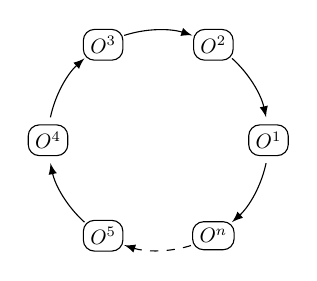
\begin{tikzpicture}[
circle/.style={
		scale=0.75,
		rounded corners,
		draw=black, 
		text centered,
		}
]

\def \n {6}
\def \m {4}
\def \radius {1.4cm}
\def \margin {12} % margin in angles, depends on the radius

\foreach \s in {1,...,\m}
{
  \node[draw, circle] at ({360/\n * (\s - 1)}:\radius) {$O^\s$};
  \draw[<-, >=latex] ({360/\n * (\s - 1)+\margin}:\radius) 
    arc ({360/\n * (\s - 1)+\margin}:{360/\n * (\s)-\margin}:\radius);
}

\node[draw, circle] at ({360/\n * 4}:\radius) {$O^5$};
  \draw[<-, dashed, >=latex] ({360/\n * 4+\margin}:\radius) 
    arc ({360/\n * 4+\margin}:{360/\n * (5)-\margin}:\radius);
    
\node[draw, circle] at ({360/\n * 5}:\radius) {$O^n$};
  \draw[<-, >=latex] ({360/\n * 5+\margin}:\radius) 
    arc ({360/\n * 5+\margin}:{360/\n * (6)-\margin}:\radius);


\end{tikzpicture}
\caption{リング決済}
\label{fig:settlement}
\end{figurehere}
\end{center}

トランザクションを生成するために、LPSCは\verb|TokenTransferDelegate|というスマートコントラクトを使用します。すべての注文が異なるバージョンのプロトコルの代わりに上記のスマートコントラクトを許可する必要があるため、このスマートコントラクトを導入することで、プロトコル内のスマートコントラクトのアップグレードが容易になります。

オーダーリングの各注文について、実装に応じて後続もしくは先行する注文に\verb|tokenS|の支払いが行われます。そして、リングマイナーの手数料は、リングマイナーが選択する手数料モデルによって選ばれます。最終的に、すべてのトランザクションが生成されたら、\verb|RingMined|イベントが送出されます。

\subsubsection{発生イベント\label{sec:events}}

プロトコルは、リレー、オーダーブラウザや、その他のアクターがオーダーブックの更新を受け取れるようにするイベントを発行します。発行されるイベントは次のとおりです。

\begin{itemize}
	\item \textbf{OrderCancelled}: 特定の注文がキャンセルされた。
	\item \textbf{OrdersCancelled}: アドレスが所有する1トレードペアのすべての注文がキャンセルされた。
	\item \textbf{AllOrdersCancelled}: アドレスが所有するすべてのトレードペアのすべての注文がキャンセルされた。
	\item \textbf{RingMined}: オーダーリングが正常に完了。このイベントにはリング内での各トークン移動に関する情報が含まれます。
\end{itemize}


\section{LRxトークン\label{sec:token}}
LRxとは我々のトークンの一般的な表記法です。LRCはEthreumでのLoopringトークンを指し、QtumではLRQ、NEOではLRNなどになります。他のLRxタイプは、今後Loopringが他のパブリックブロックチェーンに展開される際に導入されます。

\subsection{手数料モデル\label{sec:fee_model}} 
ユーザーが注文を行うとき、リングマイナーが要求できる注文に設定されたマージン(\verb|marginSplitPercentage|)の割合とともに、手数料としてリングマイナーに支払われるLRxの数量を指定します。これはマージンスプリットと呼ばれます。手数料またはマージンスプリットを選ぶかはリングマイナーに選択権があります。

マージンスプリットの説明

\begin{center}
\begin{figurehere}
\centering
\begin{tikzpicture}[
scale=1,
font=\bfseries\footnotesize\sffamily,
classical/.style={thick,<->,shorten >=2pt,shorten <=2pt,>=stealth},
oneway/.style={->,dashed,shorten >=2pt,shorten <=2pt,>=stealth}
]
    % Draw axes
    \draw [->,thick] (0,1) node (yaxis) [above] {$$}
        |- (6.2,0) node (xaxis) [right] {$$};
        
    \draw
  	(4,0) coordinate (A)
  	(4,1) coordinate (A2)
  	(4.8,-0.6) coordinate (B)
  	(4.8,1) coordinate (B2)
  	(6,-0.6) coordinate (C)
  	(6,1) coordinate (C2);
  	
  	\fill [draw=none, fill=gray!20] 
    (4.8, 0) rectangle (6, 1);
    
  	\fill [draw=none, fill=gray!10] 
    (0, -0.6) rectangle (4.8, 0);

	\draw[thick] (0, -0.6) -- (0, 0.6) node[below]{$$};
  	\draw[thick, thin] (A) -- (A2) node[below]{$$};
  	\draw[thick, thin] (B) -- (B2) node[below]{$$};
  	\draw[thick] (C) node[below, xshift=0.5cm]{$合計購入量$} -- (C2) ;
  	
  	\draw[classical] (0, 0.5) -> (4, 0.5) node[below]{$$};
  	\draw[classical] (4, 0.75) -> (4.8, 0.75) node[below]{$$};
%  	\draw[classical] (4.8, 0.5) -> (6, 0.5) node[below]{$$};
  	\draw[classical] (4, 0.25) -> (6, 0.25) node[below]{$$};

  	
  	\draw[oneway] (2, 1.2) node[above]{注文の初期購入量} -- (2, 0.5);
  	\draw[oneway] (4.4, 2.2) node[above]{追加購入量} -- (4.4, 0.75);
  	\draw[oneway] (5.4, 1.6) node[above]{マージンスプリット} -- (5.4, 1);
  	\draw[oneway] (5, -1.2) node[below]{マージン} -- (5, 0.25);
  	\draw[oneway] (2.4, -1.2) node[below]{注文の実際の購入量} -- (2.4, -0.5);



\end{tikzpicture}
\caption{60\%のマージンスプリット}
\label{fig:marginsplit}
\end{figurehere}
\end{center}

オーダーリングにおけるマージンが小さすぎる場合、リングマイナーは手数料(LRx)を選択します。逆に、マージンに余裕があり、マージンスプリットの結果がが手数料(LRx)よりも価値が大きい場合は、マージンスプリットを選択します。しかしながら、もう一つ条件があります。リングマイナーがマージンスプリットを選択した場合、リングマイナーは、ユーザー(注文作成者)がリングマイナーに支払うべき手数料(LRx)と同額を、ユーザーに支払わなければならないため、リングマイナーがマージンスプリットを選択するための閾値が、注文手数料(LRx)の2倍となり、手数料(LRx)を選択する傾向が高まります。これにより、リングマイナーは、マージンの高いオーダーリングで収入が少なくなる反面、低マージンのオーダーリングでは安定した収入を得ることができます。我々の手数料モデルは、マーケットが成長・成熟するにつれて、高いマージンのオーダーリングが少なくなり、インセンティブとして固定されたLRx手数料を必要とするという予想に基づいています。


グラフは以下のようになります。

\begin{center}
\begin{figurehere}
\centering
\begin{tikzpicture}[
font=\bfseries\footnotesize\sffamily,
oneway/.style={->,dashed,shorten >=2pt,shorten <=2pt,>=stealth},
scale=1]
    % Draw axes
    \draw [<->,thick] (0,2.7) node (yaxis) [above] {$y$}
        |- (5,0) node (xaxis) [right] {$x$};
        
    \draw
  	(1,1) coordinate (A)
  	(2,1) coordinate (B);
  	
  	
  	\draw[thick] (B) -- (3.7,2.7);
  	\draw[dotted] (B) -- (2,0) node[below] {$2f$};
  	\draw[dotted] (A) -- (1,0) node[below] {$f$};
  	\draw[thick,color=gray!70] (0,0) -- (2.7,2.7);
  	\draw[thick] (0,1) node[left] {$f$}--(B) node[     ]{$$};
 	\draw[oneway] (4,1) node[right]{マイニングの期待収益} -- (3, 2);


\end{tikzpicture}
\caption{Loopringの手数料モデル}
\label{fig:feemodel}
\end{figurehere}
\end{center}


$f$がLRx手数料、$x$がマージンスプリット、$y$がマイニング報酬です。実線で示されているように、$y=max(f, x-f)$となります。もしも注文のLRx手数料が$0$ならば、方程式は$y=max(0, x - 0)$であり、グレーの線で示されるように、単に$y=x$となります。


結果は以下のようになります。  
\begin{enumerate}
	\item マージンスプリットが0の場合、リングマイナーは、均一のLRx手数料を選択し、インセンティブを受けます。 
	\item LRx手数料が0の場合、グレー線の結果となり、報酬は通常の線形モデルに基づくことになります。
	\item マージンスプリット報酬が2x(LRx手数料)よりも大きい場合、リングマイナーはマージンスプリットを選択し、LRxをユーザーに支払います。
\end{enumerate}

LRx手数料が0でない場合、リングマイナーがどちらの選択をしようとも、リングマイナーと注文送信者との間には常にLRxの送金が発生することに注意してください。リングマイナーはLRx手数料を得るか、マージンスプリットを得るためにLRx手数料を送信者に返金します。

リングマイナーは、ウォレットと一定のパーセンテージの手数料を共有します。ユーザーがウォレットを通じて注文を行い、処理がなされると、ウォレットは手数料またはマージンスプリットの一部を報酬として受けます。これが基本的な形式ですが、独自のビジネスモデルや実施様態を構築することも可能です。獲得される手数料の約20\%から25\%をウォレットが受け取るのが我々の目指す方向です。ユーザーベースはあるものの、現状ではそれが収入源となっていることは殆どないため、ウォレットはLoopringプロトコル統合の主要ターゲットとなります。

\subsection{分散ガバナンス}
Loopringプロトコルは、メンバー間の協調に基づいて効果的に目標を達成するという意味でのソーシャルプロトコルです。これは暗号通貨経済のプロトコルと概して似ており、実際その利便性は、ゲーム理論の協力問題\cite{vitalikgovernance}、グリムトリガー均衡、限定合理性などと同じ仕組みによって守られているのです。この目的のために、LRxトークンは手数料支払いのためだけでなく、様々なネットワーク参加者の金銭的インセンティブを協調させるためにも用いられます。このような協調は、幅広く取り入れられるためにはどんなプロトコルにも必要なことですが、堅固で分散したエコシステムにおいて、流動性を向上させることが成功への大きな鍵となる取引所プロトコルでは殊更に重要となります。

LRxトークンは、分散ガバナンスでのプロトコルのアップデートを実現するために使われます。スマートコントラクトのアップデートは、連続性と安全性を保ち、不整合性による流動性の低下リスクを少なくするために、トークンホルダーによるガバナンスが部分的に行われます。スマートコントラクトは一度デプロイされると変更ができないため、dAppsやエンドユーザーが廃止予定のバージョンと相互作用し続け、アップデートされたコントラクトから適合外となるリスクがあります。市場の需要と新たなブロックチェーンに適応しなければならないため、アップグレード可能であることがプロトコルの成功には不可欠です。LRxホルダーによる分散ガバナンスは、dAppsやエンドユーザーに影響を与えたり、スマートコントラクトの抽象化に過度に依存することなく、プロトコルのアップデートを可能にします。LRxトークンは供給量が固定されており、LRCの場合には、一定割合がLoopring財団によって凍結されており、コミュニティ指向のファンドに割り当てられます\cite{LRCtokendoc}。

しかしながら、LRxのトークン所有者のみが、プロトコルの方向性を左右するステークホルダーなのではありません。リレー、リングマイナー、ウォレット、開発者等は皆、エコシステムに不可欠な存在であり、その声は聞かれなければなりません。実際、これらの存在は、それぞれの役割を果たすためにLRxを保持する必要はなく(従来のメーカー/テイカーとマーケットメーカーは存在しないため、初期のトークンリザーブは必須ではありません)他の方法によって、彼らの利益を尊重しなければなりません。さらに言えば、「単純な」トークンベースの投票は、低い投票率とトークン保持者の偏在性がリスクを生むため、オンチェーン・オフチェーンを問わず、合意不成立への対処としては不完全です。したがって、最終的なゴールはレイヤー上にガバナンスモデルを構築することであり、何らかの意思決定プロセスを規範とする共有知識に、この成否がかかっています。これは、幅広い参加者からのシグナルと、ことによればまだ確立していないプロトコルの焦点からのシグナルを提供する協力機関によって促進されます。分散ガバナンスが実現するにつれて、Loopring財団は必然的に、プロトコルの開発者から、プロトコルの世話役となるでしょう。

\section{詐欺と攻撃への耐性}

\subsection{フロントランニング防止\label{sec:dual_authoring}}

分散型取引所においてのフロントランニングとは、他のノードのトレードソリューションをコピーし、未処理のトランザクションプール(メモリプール)にある元々のトランザクションよりも前にマイニング承認を済ませることです。これは、より高い取引手数料(ガス価格)を指定することで起こりえます。Loopring(といかなるオーダーマッチングのプロトコル)でのフロントランニングの主な手法は、オーダーフィルチ(フロントランナーが未処理のオーダーリング決済トランザクションから、1つあるいは複数の注文を盗むこと。Loopringに限れば、フロントランナーが未処理のオーダーリング全体を盗むこと)です。

submitRingトランザクションが承認されないまま、未処理のトランザクションプールに残っている場合、誰でもそのトランザクションを見つけ、\verb|minerAddress|を自分のアドレス(\verb|filcherAddress|)に変更し、\verb|filcherAddress|でペイロードを放棄させ、オーダーリングの署名を書き換えることができます。フィルチャーは、ブロックマイナーが元のsubmitRingトランザクションではなく、フィルチャーのトランザクションを次のブロックに記録することを期待して、より高いガス価格を設定したトランザクションを新たに送信することができます。

この問題への従来の解決策には重大な弱点がありました。追加のトランザクションを必要とするため、リングマイナーに多くのガス負担をかけ、オーダーリングの決済に最低でも2倍のブロックを使用することです。我々の新たな解決策であるデュアル認証\cite{dualauthor}では、注文に2段階の認証(決済段階とリングマイニング段階)を設定する仕組みを採用しています。

デュアル認証プロセス

\begin{enumerate}

	\item 各注文に対し、ウォレットソフトウェアはランダムな公開鍵/秘密鍵のペアを生成し、注文のJSONスニペット内に配置します。(あるいは、バイトサイズを小さくするために、公開鍵自体ではなく公開鍵に紐づいたアドレスを使用できます。このようなアドレスを表すのに\verb|authAddr|を使用し、対応する秘密鍵を表すのに\verb|authAddr|を使用します)

	\item 注文に含まれる全てのフィールド(\verb|r|, \verb|v|, \verb|s|および\verb|authKey|を除く)で注文のハッシュを計算し、所有者の秘密鍵(\verb|authKey|ではなく)を使ってハッシュに署名します。

	\item ウォレットは\verb|authKey|と合わせて注文をリングマイニング用のリレーに送ります。リングマイナーは、\verb|authKey|と\verb|authAddr|が正しくペアになっていることと、オーダーの署名が所有者アドレスに対して有効であることを検証します。

	\item オーダーリングが識別されると、リングマイナーは各注文の\verb|authKey|を使用して、リングのハッシュ、\verb|minerAddress|、その他全てのマイニングパラメータに署名します。オーダーリングに$n$個の注文が含まれている場合、$n$個の\verb|authKey|による$n$個の署名が存在し、これらの署名を\verb|authSignature|と呼びます。リングマイナーは\verb|minerAddress|の秘密鍵を使用して、全てのマイニングパラメータとともにリングのハッシュに署名をする必要があります。

	\item リングマイナーは全てのパラメータと全ての余分な\verb|authSignature|を使用してsubmitRing関数を呼び出します。\verb|authKey|はオンチェーンのトランザクションの一部分ではなく、リングマイナー以外の第三者には明かされないことに注意してください。

	\item Loopringプロトコルは各注文の対応する\verb|authAddr|に対して各\verb|authSignature|を検証し、\verb|authSignature|が不足または無効なオーダーリングを拒否します。
 
\end{enumerate}

その結果は以下のようになります。

\begin{itemize}

	\item  注文の(所有者アドレスの秘密鍵による)署名は、\verb|authAddr|を含め、注文の変更が不可能であることを保証します。
	\item  リングマイナーの(\verb|minerAddress|の秘密鍵による)署名が提供された場合は、マイナーのアイデンティティを使用してのオーダーリングのマイニング承認が不可能であることを保証します。
	\item  \verb|authSignature|は、\verb|minerAddress|を含め、オーダーリング全体の変更、および注文の盗難が不可能であることを保証します。

\end{itemize}

デュアル認証はリングフィルチとオーダーフィルチを防止し、オーダーリングの決済がひとつのトランザクション内で行われることを保証します。さらに、デュアル認証は、非マッチ共有・マッチ共有という2つの方法でリレーが注文を共有することを可能にします。デフォルトでは、LoopringはOTCモデルで稼働し、指値注文のみをサポートし、注文のタイムスタンプは無視されます。よって、フロントランニングは、実際の取引価格には影響しませんが、取引が処理されるか否かには影響を及ぼすことを意味します。

\section{オーダー攻撃}

\subsection{シビル攻撃およびDOS攻撃}
悪意あるユーザー(当人としてふるまおうと別人になりすまそうと)は、規模の小さい注文を大量に送り、Loopringノードへの攻撃を試みるかもしれません。しかしながら、ノードはそれぞれの基準(公開および非公開)に基づいて注文を拒否することができるため、このような注文のほとんどは、マッチしたとしても、十分な利益を生みださないとして拒否されます。注文を管理するリレーの権限を強化することで、小規模かつ多量のオーダー攻撃は脅威となりません。

\subsection{不十分な残高}
悪意のあるユーザーが、アドレスの実際の残高がゼロにもかかわらず、注文価値がゼロではない注文に署名をして広めることができます。ノードは、実際の残高がゼロの注文を監視して発見することができ、それらの注文ステータスを更新し破棄することができます。ノードは注文ステータスを更新するために時間を消費しますが、アドレスのブラックリスト化や関連する注文の破棄を行うことで、コストを最小限に抑えることもできます。

\section{要約}

Loopringプロトコルは分散型取引所のための基盤となることを目指しています。そうすることで、人々が資産や価値をどのように交換するかに大きな影響を与えるでしょう。中間商品として、お金は物々交換を容易にしたり、または置き換え、二重の要求の一致問題\cite{unenumerated2006}を解決します、これは二つのグループがお互い別々のモノを求めなければならないという状況による問題です。同じように、Loopringプロトコルは、より簡単に取引を簡潔させるリングマッチングを用いて、取引ペアにおける要求の一致の信頼度を分配することを狙っています。これは、社会やマーケットがトークンや従来の資産などを、どのように交換するかについて意味のあるものです。確かに、分散型の暗号通貨は国家のお金に対する支配権を脅かすように、トレーダー(消費者と生産者)同士を結び付ける複合的なプロトコルは、お金の概念そのものへの理論上の脅威となります。

プロトコルは以下の利点をユーザーに与えます。

\begin{itemize}
	\item オフチェーンのオーダー管理とオンチェーンでの決済は安全性を犠牲にすることはありません。
	\item リングマイニングとオーダーシェアリングによるより高い流動性。
	\item 二重認証は現在の全てのDEXとそのユーザーが直面するフロントランニングの悪質な問題を解決します。
	\item 自由かつパブリックなスマートコントラクトはいかなるdAppsでも、プロトコル上に構築または操作することを可能にします。
	\item 事業者間の標準化により、ネットワーク効果とエンドユーザー体験の向上が可能になります。
	\item ネットワークはオーダーブックの運用と伝達での柔軟性とともに維持されます。
	\item 参加への障壁が減るということは、ノードとエンドユーザがネットワークに参加するためのコストが低いということを意味します。
	\item ユーザーウォレットからの直接の匿名取引。
\end{itemize}

\section{謝辞}
メンターやアドバイザー、そして私たちを歓迎してくれた有識なたくさんのコミュニティメンバーに感謝いたします。特に、我々のプロジェクトに関してのレビューをいただいたShuo Bai氏(ChinaLedger)、Habin Kan教授、Alex Cheng氏、Hongfei Da氏、Yin Cao氏、Xiaochuan Wu氏、Zhen Wang氏、Wei Yu氏、Nian Duan氏、Jun Xiao氏、Jiang Qian氏、Jiangxu Xiang氏、Yipeng Guo氏、Dahai Li氏、Kelvin Long氏、Huaxia Xia氏、Jun Ma氏、Encephalo Path氏に感謝申し上げます。


\bibliography{whitepaper}
\bibliographystyle{unsrt}


\end{multicols}


\begin{appendices}

\section{イーサリウム上のLoopring\label{app:protocol_ethereum}}

\subsection{スマートコントラクト}

\begin{center}
\begin{figurehere}
\centering
\begin{tikzpicture}
[node distance = 1cm, auto,font=\footnotesize,
% STYLES
every node/.style={node distance=3cm},
% The comment style is used to describe the characteristics of each force
comment/.style={rectangle, inner sep= 5pt, text width=4cm, node distance=0.25cm, font=\scriptsize\sffamily},
% The force style is used to draw the forces' name
force/.style={rectangle, draw, fill=black!10, inner sep=5pt, text width=4cm, text badly centered, minimum height=1.2cm, font=\bfseries\footnotesize\sffamily}] 

% Draw forces
\node [force] (impl) {LoopringProtocolImpl};
\node [force, dashed, above of=impl] (protocol_interface) {LoopringProtocol};
\node [force, left=1cm of impl] (nameregistry) {NameRegistry};
\node [force, right=1cm of impl] (tokenregistry) {TokenRegistry};
\node [force, below of=impl] (delegate) {TokenTransferDelegate};
\node [force, left=1cm of delegate] (multisig) {TransferableMultsig};

%%%%%%%%%%%%%%%
% Change data from here

% impl
\node [comment, below=0.25 of impl] (comment-impl) {- オーダーリングを検証する\\
- 決済用にトークンを転送\\
- イベントを発生する};

% nameregistry
\node [comment, below=0.25cm of nameregistry]{- ウォレットとリレーを登録する};

% protocol_interface
\node [comment, below=0.25 of protocol_interface](comment-interface) {- インターフェースとイベントを定義する};

% tokenregistry
\node [comment, below=0.25 of tokenregistry] {- ERC20/ERC223トークンを登録する};

% delegate
\node [comment, below=0.25 of delegate] {- ユーザーに代わりトークンを転送する};

% PUBLIC POLICIES
\node [comment, text width=3cm, below=0.25 of multisig] {- マルチシグオーナーシップを実現する};

%%%%%%%%%%%%%%%%

% Draw the links between forces
\path[->,thick] 
(comment-interface) edge (impl)
(nameregistry) edge (impl)
(tokenregistry) edge (impl)
(delegate) edge (comment-impl);

\end{tikzpicture} 
\caption{スマートコントラクト}
\label{fig:smartcontracts}
\end{figurehere}
\end{center}

\subsection{デプロイメント}

以下のスマートコントラクトはイーサリアムメインネット上にデプロイされています。
\begin{itemize}
\item LRC: \verb|0xEF68e7C694F40c8202821eDF525dE3782458639f|
\item TokenRegistry: \verb|0xa21c1f2AE7f721aE77b1204A4f0811c642638da9|
\item TokenTransferDelegate: \verb|0xc787aE8D6560FB77B82F42CED8eD39f94961e304|
\item NameRegistry: \verb|0x0f3Dce8560a6010DE119396af005552B7983b7e7|
\item LoopringProtocolImpl: \verb|0xc80BbAb86cED62CF795619A357581FaF0cB46511|
\item TransferableMultsig: \verb|0x7421ad9C880eDF007a122f119AD12dEd5f7C123B|
\end{itemize}

\end{appendices}
\end{document}
